\def\SigmaBlob{plot[smooth cycle,tension=0.7] coordinates {(-3.2,0.1) (-2.6,0.9) (-1.2,1.7) (0.8,1.9) (2.6,1.5) (3.3,0.4) (2.8,-0.9) (1.0,-1.5) (-1.4,-1.4) (-3.0,-0.8)}}

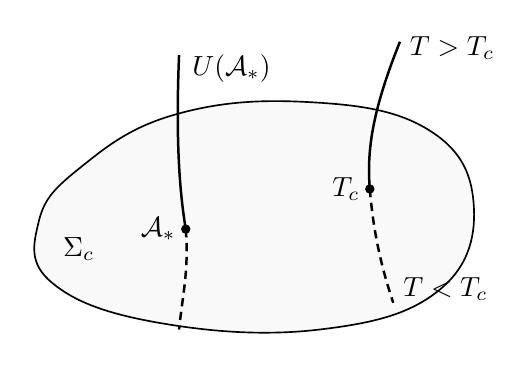
\begin{tikzpicture}[line width=0.6pt,scale=0.85]
  \draw[fill=gray!5] \SigmaBlob;
  \node at (-2.6,-0.3) {$\Sigma_c$};
  \draw[line width=0.9pt] (-1.1,2.6) .. controls (-1.15,1.4) and (-1.1,0.6) .. (-1.0,0.0);
  \draw[line width=0.9pt,densely dashed] (-1.0,0.0) .. controls (-0.95,-0.6) and (-1.05,-1.0) .. (-1.1,-1.5);
  \fill (-1.0,0.0) circle (2pt) node[left] {$\mathcal A_*$};
  \node[right] at (-1.05,2.4) {$U(\mathcal A_*)$};
  \draw[line width=0.9pt] (2.2,2.8) .. controls (1.8,1.8) and (1.7,1.2) .. (1.75,0.6);
  \draw[line width=0.9pt,densely dashed] (1.75,0.6) .. controls (1.8,0.0) and (1.9,-0.5) .. (2.1,-1.1);
  \fill (1.75,0.6) circle (2pt) node[left] {$T_c$};
  \node[right] at (2.2,2.7) {$T>T_c$};
  \node[right] at (2.1,-0.9) {$T<T_c$};
\end{tikzpicture}
